\documentclass[a4paper, 12pt]{report}
\usepackage[utf8]{inputenc}
\usepackage{geometry}
\usepackage{polski}
\usepackage{graphicx}
\usepackage{float}
\usepackage{etoolbox,refcount}
\usepackage{multicol}
\usepackage{amsmath}
\usepackage{hyperref}

\newgeometry{left=2cm, right=2cm, bottom=1.5cm, top=1.5cm}
\author{Adrian Jałoszewski, Tomasz Kotowski,\\ Dorota Kowalik, Michał Krent}
\title{Model kinematyki samochodu demonstracyjnego EVE i jego identyfikacja -- raport}
\date{9 maja 2016}
\begin{document}
	\maketitle
	\tableofcontents
	\newpage
	\chapter{Model matematyczny}
		\section{Sterowanie Ackermana}
			Do naszych zastosowań wybraliśmy sterowanie Ackermana. Jest to model specjalnie stworzony pod sterowanie pojazdami, które posiadają koła skrętne. Aby jednak móc sterować tym pojazdem musieliśmy tak dobrać punkty okręgu po którym nastąpiłoby przemieszczenie, aby jego tylna oś była prostopadła do okręgu po którym się przemieszcza.
			\begin{figure}[H]
				\centering
				\includegraphics[width = 0.6\textwidth]{./img/ackerman.png}
				\caption{Sterowanie Ackermana}
			\end{figure}
			\noindent Punktami gwarantującymi, że tak będzie jest dowolny punkt samochodu nie leżący na tylnej osi oraz jego odbicie względem tej osi. Trzecim punktem potrzebnym do wyznaczenia okręgu po którym będzie się poruszał pojazd jest kolejny punkt, w którym ma się znaleźć uprzednio wybrany punkt samochodu. Ponieważ naszym celem jest symulacja ruchu środka ciężkości pojazdu, to tym punktem samochodu będzie jego środek ciężkości. 
			\newline
			\newline
			Pomiary samochodu potrzebne do modelu Ackermanna:
			\begin{itemize}
				\item[--] odległość między osią tylną, a przednią: 1,8 m
				\item[--] rozstaw osi: 143,5 cm
				\item[--] szerokość: 55 cm
				\item[--] skrętność kół $15^o$--$18^o$ (problemy z precyzyjnym zmierzeniem) 
			\end{itemize}
		\section{Kinematyka prosta}
			Celem kinematyki prostej jest wyznaczenie poruszania się pojazdu w zależności od zastosowanego na nim sterowania. W naszym przypadku jako sterowanie przyjmujemy wartość kąta na lewym kole, gdyż nie ma potrzeby generowania tych wartości dla dwóch kół -- łączy je sztywna zależność. Dla uproszczenia założyliśmy, że samochód porusza się ze stałą prędkością -- używamy stałego kroku o długości 10 cm. Samochód zaczyna swoją trasę z punktem nr 4 w punkcie (0.0), skierowany zgodnie z wektorem (0,1).
			\newline
			\newline
			Wyznaczanie kinematyki prostej rozpoczynamy od przeniesienia punktu nr 4 pojazdu do środka układu współrzędnych. 
			\begin{figure}[H]
				\centering
				\includegraphics[height=8cm,width=0.4\textwidth]{./img/1.png}
				\includegraphics[height=8cm,width=0.4\textwidth]{./img/2.png}
			\end{figure}
			\noindent Następnie dokonujemy obrotu w celu wyprostowania samochodu i w układzie związanym \linebreak z samochodem wyznaczamy środek obrotu z zależności trygonometrycznych, a następnie dokonujemy obrotu odwrotnego do tego, co go uprzednio wykonaliśmy.
			\begin{figure}[H]
				\centering
				\includegraphics[height=8cm, width=0.4\textwidth]{./img/3.png}
				\includegraphics[height=8cm, width=0.4\textwidth]{./img/4.png}
			\end{figure}
			\noindent Należy następnie cofnąć translację, wracając do układu globalnego związanego z podłożem, a następnie dokonać translacji do układu, którego środkiem jest uprzednio wyznaczony środek obrotu.
			\begin{figure}[H]
				\centering
				\includegraphics[height=8cm, width=0.4\textwidth]{./img/5.png}
				\includegraphics[height=8cm, width=0.4\textwidth]{./img/6.png}
			\end{figure}
			\noindent Ostatnimi dwoma krokami jest obrót samochodu względem środka obrotu o 10 centymetrów \linebreak i powrót do układu globalnego.
			\begin{figure}[H]
				\centering
				\includegraphics[height=8cm, width=0.4\textwidth]{./img/7.png}
				\includegraphics[height=8cm, width=0.4\textwidth]{./img/8.png}
			\end{figure}
			\noindent Ze względu na dokonywane translacje, wszystkie zastosowane rotacje względem punktu są przekształceniami liniowymi wektorów, a dodanie kolejnego wymiaru wypełnionego jedynkami do wektorów zamienia również translacje w przekształcenia liniowe. Pozwala to na zastosowanie macierzy obrotu i macierzy translacji do wszystkich manipulacji.
			\newline
			\newline
			Oddzielnie należy potraktować przypadek kiedy koła są wyprostowane -- wtedy należy przesunąć samochód o zadany wektor o długości 10 centymetrów zgodnie z kierunkiem ruchu.
			\newline 
			\newline
			Całokształt operacji można zapisać jako:
			$$
				X_{n+1} = T_{Rn}^{-1}R_{Rn}T_{Rn}T_{1n}^{-1}R_{1n}^{-1}\mathrm{\{obliczenia\}}R_{1n}T_{1n} X_{n}
			$$
			Gdzie $T_{Rn}$ to macierz translacji przesuwająca środek obrotu do środka układu współrzędnych, macierz $R_{Rn}$ to macierz obrotu o dany kąt (tak aby przesunąć o 10 cm), macierz $T_{1n}$ to macierz translacji sprowadzająca środek tylnej osi do środka układu współrzędnych, a $R_{1n}$ to macierz dokonująca rotacji prostującej samochód. Obliczenia mają na celu wyznaczenie środka obrotu i dokonania na nim pozostałych przekształceń.
		\newpage
		\section{Kinematyka odwrotna}
			Zadaniem kinematyki odwrotnej jest wyznaczenie sterowania na podstawie zadanej ścieżki po jakiej się porusza pojazd. Podobnie jak w kinematyce prostej przyjmujemy tu jako źródło sterowania lewe koło.
			\newline
			\newline
			Całość należy rozpocząć od wyznaczenia środka obrotu lub podania kąta $0^o$ w wypadku jeżeli ten środek nie istnieje (jedziemy linią prostą). Do wyznaczenia tego używamy następującego układu równań:
			$$
				\left\{\begin{matrix}
					(x_1-a)^2 + (y_1-b)^2 = r^2 \\ 
					(x_2-a)^2 + (y_2-b)^2 = r^2 \\ 
					(x_3-a)^2 + (y_3-b)^2 = r^2
				\end{matrix}\right.
			$$
			Gdzie $(a,b)$ to środek okręgu po którym ma się poruszać środek ciężkości, a $r$ to jego promień. Można to inaczej zapisać jako:
			$$
				\begin{bmatrix}
					2x_1-2x_3 & 2y_1-2y_3\\ 
					2x_2-2x_3 & 2y_2-2y_3 
				\end{bmatrix}
				\cdot
				\begin{bmatrix}
					a\\ 
					b
				\end{bmatrix}
				=
				\begin{bmatrix}
					x_1^2 - x_3^2 + y_1^2-y_3^2\\
					x_2^2 - x_3^2 + y_2^2-y_3^2 
				\end{bmatrix}
			$$
			Odpowiednie punkty to:
			\begin{itemize}
				\item[] $(x_1,y_1)$ -- środek masy
				\item[] $(x_2,y_2)$ -- odbicie symetryczne środka masy względem tylnej osi
				\item[] $(x_3,y_3)$ -- kolejny punkt trasy
			\end{itemize}
			Jeżeli wyznacznik macierzy jest równy zero, to znaczy, że poruszamy się po prostej, w przeciwnym wypadku wyznaczamy przy pomocy iloczynu wektorowego i skalarnego potrzebny nam kąt i dokonujemy obrotu na samochodzie do następnego punktu.
			$$
				X_{n+1} = T_{Rn}^{-1}R_{Rn}T_{Rn} X_{n}
			$$
			$T_{Rn}$ to macierz przesuwająca punkt obrotu do środka układu współrzędnych, a macierz $R_{Rn}$ to macierz dokonująca obrotu o zadany kąt. W obliczeniach iloczyn skalarny służy nam do wyznaczenia wartości kąta (arcus cosinus ma odpowiedni zakres), a iloczyn wektorowy służy do określania kierunku obrotu.
		\section{Reprezentacja pojazdu autonomicznego EVE}
			Pojazd autonomiczny EVE jest reprezentowany macierzą:
			$$
				\begin{bmatrix}
					x_1 & x_2 & x_3 & x_4 & x_5 & x_6 & x_7 & x_8 \\ 
					y_1 & y_2 & y_3 & y_4 & y_5 & y_6 & y_7 & y_8 \\ 
					1 & 1 & 1 & 1 & 1 & 1 & 1 & 1
				\end{bmatrix}
			$$
			Gdzie $(x_i,y_i)$ to odpowiednie punkty oznaczone zgodnie ze schematem w podpunkcie o sterowaniu Ackermana.
	\chapter{Implementacja}
		\section{Kinematyka prosta}
			\begin{figure}[H]
				\centering
				\includegraphics[width = \textwidth]{./img/fwd.png}
				\caption{Kinematyka prosta}
			\end{figure}
		\section{Kinematyka odwrotna}
			\begin{figure}[H]
				\centering
				\includegraphics[width = \textwidth]{./img/inv.png}
				\caption{Kinematyka odwrotna}
			\end{figure}
			W zadaniu kinematyki odwrotnej mieliśmy dodatkowo sprawdzić, czy pojazd mieści się w zadanych ograniczeniach oraz czy manewr jest wykonywalny. W przypadku kiedy manewr jest awykonalny lub nie da się go wykonać w polu wyznaczonym do manewru (wielokąt), to wyskakuje okno dialogowe i przerywa działanie skryptu zwracając do tej pory wyznaczone wartości.
			\newline
			\newline 
			W przypadku jakby się chciało podobny efekt uzyskać dla kinematyki prostej należy wynik z obliczeń kinematyki prostej przeprowadzić przez funkcję kinematyki odwrotnej.
			\newline 
			\newline
			Funkcja rozpoczyna swoje działanie od utworzenia i umieszczeniu pojazdu na trasie.
		\section{Funkcje pomocnicze}
			\subsection{Macierz rotacji i translacji}
				\begin{figure}[H]
					\includegraphics[width = 0.6\textwidth]{./img/rot_tran.png}
				\end{figure}
			\subsection{Tworzenie pojazdu autonomicznego macierzy EVE}
				\begin{figure}[H]
					\includegraphics[width = 0.45\textwidth]{./img/eve.png}
				\end{figure}
			\subsection{Iloczyn skalarny, wektorowy, długość wektora, kąt między wektorami}
				\begin{figure}[H]
					\includegraphics[width = 0.6\textwidth]{./img/pdla.png}
				\end{figure}
			\subsection{Wyznaczenie środka okręgu}
				\begin{figure}[H]
					\includegraphics[width = 0.4\textwidth]{./img/centr.png}
				\end{figure}
	\chapter{Testy}
		Testy są podzielone na dwie kategorie, ze względu na to, jakie funkcje miały za zadanie sprawdzić. Jednak każda z kategorii testów zawiera w sobie od razu przykłady testów z drugiej kategorii, gdyż wyjście z jednej funkcji mogło służyć jako wejście do innej. Ponieważ zadanie kinematyki prostej jest odwrotne do zadania kinematyki odwrotnej mogliśmy w ten sposób dokonać walidacji wyników, gdyż przepuszczając najpierw serię kątów przez funkcję odpowiedzialną za kinematykę prostą mogliśmy wynik z niej wykorzystać jako wejście do kinematyki odwrotnej.
		\newline 
		\newline
		Ponieważ jest bardzo mało prawdopodobne, że obydwie funkcje zostały wykonane wadliwie w ten sposób aby wady z jednej funkcji znosiły się z wadami z drugiej funkcji uznaliśmy to za wiarygodny sposób walidacji poprawności naszych funkcji. Jednak ze względu na to, że krok stały jest szczególnym przypadkiem kroku zmiennego działa to tylko w jedną stronę -- z kinematyki prostej, gdzie mieliśmy krok stały, wynoszący 10 cm. w kinematykę odwrotną.
		\newline 
		\newline
		Mechanizm testów został przez nas w pełni zautomatyzowany tak aby z łatwością móc włączać \linebreak i wyłączać testy przez wykomentowanie odpowiednich linii. Wyłączanie testów jest koniecznością ze względu na ich czasochłonność -- każdy test dokonywał zapisu na dysku trzech wykresów. Jest to przez nas stworzony mechanizm testów jednostkowych, pozwalający nam na tworzenie naszych funkcji na zasadach TDD. Ponieważ kod odpowiedzialny za sprawdzanie czy pojazd znajduje się w konturze jest funkcją wbudowaną MATLABa, postanowiliśmy go nie testować.
		\begin{figure}[H]
			\centering
			\includegraphics[width = 0.6\textwidth]{./codes/test_suite.png}
		\end{figure}
		\section{Kinematyka Prosta}
			Wyniki testów to trzy wykresy. Pierwszy pokazuje ścieżkę wyznaczoną przy pomocy kinematyki prostej, drugi przedstawia ścieżkę zakreśloną przez środek masy w trakcie wykonywania obliczeń dla kinematyki odwrotnej, a trzeci przedstawia kąty w stopniach, jakie zostały zwrócone przez funkcję kinematyki odwrotnej w zależności od iteracji. Pierwsze dwa przebiegi są wyskalowane w metrach.
			\newline
			\newline
			\noindent Poniższy fragment kodu przedstawia schemat jakim się kierowaliśmy przy tworzeniu naszych testów jednostkowych dla kinematyki prostej. Dokonywał on inicjalizacji danych wejściowych w postaci wektora o długości $n$, a następnie przekazywał je do funkcji odpowiedzialnej za kinematykę prostą. Stamtąd były pobierane dane w postaci macierzy $3\times n$ i przekazywane do funkcji odpowiedzialnej za kinematykę odwrotną.
			\begin{figure}[H]
				\centering
				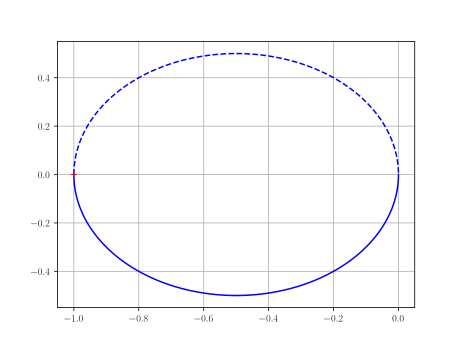
\includegraphics[width = 0.6\textwidth]{./codes/test.png}
			\end{figure}
			\noindent Taki pojedynczy test dawał nam w odpowiedzi trzy wykresy, które były następnie zapisywane na dysku i były dostępne do ręcznego porównania.
			\newline
			\newline
			Z początku przebiegów kąta w funkcji iteracji można dosyć często zauważyć różne wartości, które mogą się zdawać niezgodne z przewidywaniami teoretycznymi. Nie jest to jednak ani błąd symulacji, ani błąd modelu -- efekt ten bierze się stąd, że zgadzać się ma położenie środka ciężkości, a kierunek pojazdu nie musi być styczny do trasy po której pojazd miałby się poruszać. Jednak po pewnym czasie pojazd się stabilizuje i zaczyna poprawnie śledzić ścieżkę tak, aby kierunek jego pokrywał się ze styczną do toru.
			\newpage
			\subsection{Sinusoida}
				Obydwie ścieżki są ze sobą zgodne. Po kształcie krzywych można rozpoznać, że zachowują się jakby na wejściu miały zadaną pewną sinusoidę.
				\begin{figure}[H]
					\centering
					\includegraphics[width = 0.8\textwidth]{./AP/img/sin_in_1.png}
					\caption{Ścieżka wyznaczona przez kinematykę prostą}
				\end{figure}
				\begin{figure}[H]
					\centering
					\includegraphics[width = 0.8\textwidth]{./AP/img/sin_in_2.png}
					\caption{Ścieżka którą podążał pojazd}
				\end{figure}
				\begin{figure}[H]
					\centering
					\includegraphics[width = 0.8\textwidth]{./AP/img/sin_in_3.png}
					\caption{Kąt wyznaczony przez kinematykę odwrotną}
				\end{figure}
				\noindent Ponieważ na wyjściu otrzymaliśmy tę samą sinusoidę z drobnymi zawahaniami w początkowych fazach (pojazd musiał ustawić się na torze) wnioskujemy, że test został przeprowadzony poprawnie.
			\newpage
			\subsection{Skok zadany, dodatni}
				Obydwie ścieżki są ze sobą zgodne. Zgodnie z przewidywaniami są to okręgi (kąt skrętu był stały), które zaczynają się w punkcie (0,0). Samochód poruszał się po nich zgodnie z dodatnim kierunkiem trygonometrycznym po okręgu o promieniu zgodnym z przewidywaniami.
				\begin{figure}[H]
					\centering
					\includegraphics[width = 0.8\textwidth]{./AP/img/step_1_in_1.png}
					\caption{Ścieżka wyznaczona przez kinematykę prostą}
				\end{figure}
				\begin{figure}[H]
					\centering
					\includegraphics[width = 0.8\textwidth]{./AP/img/step_1_in_2.png}
					\caption{Ścieżka którą podążał pojazd}
				\end{figure}
				\begin{figure}[H]
					\centering
					\includegraphics[width = 0.8\textwidth]{./AP/img/step_1_in_3.png}
					\caption{Kąt wyznaczony przez kinematykę odwrotną}
				\end{figure}
				\noindent Na wykresie pozyskanym z kinematyki odwrotnej można zauważyć fazę początkową jak pojazd próbuje wjechać na koło i na nim pozostać (nierówne ustawienie go na początku linii) oraz to, że kąt ten po ustabilizowaniu się jest równy kątowi, który został zadany w teście.
			\newpage
			\subsection{Skok zadany, ujemny}
				Obydwie ścieżki są ze sobą zgodne. Zgodnie z przewidywaniami są to okręgi (kąt skrętu był stały), które zaczynają się w punkcie (0,0). Samochód poruszał się po nich zgodnie z ujemnym kierunkiem trygonometrycznym po okręgu o promieniu zgodnym z przewidywaniami.
				\begin{figure}[H]
					\centering
					\includegraphics[width = 0.8\textwidth]{./AP/img/step_2_in_1.png}
					\caption{Ścieżka wyznaczona przez kinematykę prostą}
				\end{figure}
				\begin{figure}[H]
					\centering
					\includegraphics[width = 0.8\textwidth]{./AP/img/step_2_in_2.png}
					\caption{Ścieżka którą podążał pojazd}
				\end{figure}
				\begin{figure}[H]
					\centering
					\includegraphics[width = 0.8\textwidth]{./AP/img/step_2_in_3.png}
					\caption{Kąt wyznaczony przez kinematykę odwrotną}
				\end{figure}
				\noindent Na wykresie pozyskanym z kinematyki odwrotnej można zauważyć fazę początkową jak pojazd próbuje wjechać na koło i na nim pozostać (nierówne ustawienie go na początku linii) oraz to, że kąt ten po ustabilizowaniu się jest równy kątowi, który został zadany w teście.
			\newpage
			\subsection{Proces gaussowski}
				W tym teście wektorem wprowadzonym przez nas na wejście jest proces gaussowski taki, że każdy kolejny krok jest punktem spełniającym rozkład normalny przekształcony w pewien sposób ograniczający jego wartość do dopuszczalnego zakresu. Obydwie ścieżki są ze sobą zgodne.
				\begin{figure}[H]
					\centering
					\includegraphics[width = 0.8\textwidth]{./AP/img/random_gauss_in_1.png}
					\caption{Ścieżka wyznaczona przez kinematykę prostą}
				\end{figure}
				\begin{figure}[H]
					\centering
					\includegraphics[width = 0.8\textwidth]{./AP/img/random_gauss_in_2.png}
					\caption{Ścieżka którą podążał pojazd}
				\end{figure}
				\begin{figure}[H]
					\centering
					\includegraphics[width = 0.8\textwidth]{./AP/img/random_gauss_in_3.png}
					\caption{Kąt wyznaczony przez kinematykę odwrotną}
				\end{figure}
				\noindent Pomimo tego, że kąt który był wykorzystywany do testu był z zakresu (-11,5, 11,5) stopni można na przebiegu zauważyć, że wartość ta jest nieco przekraczana. Proces gaussowski dla wartości bliższych maksymalnego zakresu kąta doprowadzał do wyskoczenia komunikatu o przekroczeniu maksymalnego zakresu. Są to jednak błędy numeryczne wynikające z liczby iteracji.
			\newpage
			\subsection{Wartości losowe dodatnie}
				Ścieżki zgadzają się ze sobą. Pojazd porusza się zgodnie z dodatnim kierunkiem trygonometrycznym po różnych krągłych krzywych. Dzieje się tak ponieważ zmieniając losowo kąt zmienia się również losowo środek obrotu, jednak wartości tylko dodatnie gwarantują, że obrót będzie się zawsze odbywać w dodatnim kierunku trygonometrycznym.
				\begin{figure}[H]
					\centering
					\includegraphics[width = 0.8\textwidth]{./AP/img/random_right_in_1.png}
					\caption{Ścieżka wyznaczona przez kinematykę prostą}
				\end{figure}
				\begin{figure}[H]
					\centering
					\includegraphics[width = 0.8\textwidth]{./AP/img/random_right_in_2.png}
					\caption{Ścieżka którą podążał pojazd}
				\end{figure}
				\begin{figure}[H]
					\centering
					\includegraphics[width = 0.8\textwidth]{./AP/img/random_right_in_3.png}
					\caption{Kąt wyznaczony przez kinematykę odwrotną}
				\end{figure}
				\noindent Na podstawie rozkładu wartości kąta, jaki sczytała kinematyka odwrotna można zauważyć funkcję, która była przez nas używana do ograniczenia wartości zmiennej losowej. Używaliśmy do tego tangensa hiperbolicznego, który generuje zagęszczenie występowania wartości wyższych. Na podstawie tego i ścieżki którą podążał pojazd możemy stwierdzić, że test został zakończony poprawnie.
			\newpage
			\subsection{Wartości losowe ujemne}
				Ścieżki zgadzają się ze sobą. Podobnie jak dla wartości losowych dodatnich krzywe są krągłe. Jednak w tym przypadku mają ujemny kierunek trygonometryczny -- pojazd porusza się zgodnie ze wskazówkami zegara.
				\begin{figure}[H]
					\centering
					\includegraphics[width = 0.8\textwidth]{./AP/img/random_left_in_1.png}
					\caption{Ścieżka wyznaczona przez kinematykę prostą}
				\end{figure}
				\begin{figure}[H]
					\centering
					\includegraphics[width = 0.8\textwidth]{./AP/img/random_left_in_2.png}
					\caption{Ścieżka którą podążał pojazd}
				\end{figure}
				\begin{figure}[H]
					\centering
					\includegraphics[width = 0.8\textwidth]{./AP/img/random_left_in_3.png}
					\caption{Kąt wyznaczony przez kinematykę odwrotną}
				\end{figure}
				\noindent Odczytane wartości kątów zgadzają się z tymi zadanymi. Z początku jednak można zauważyć krótką chwilę kiedy samochód poruszał się w kierunku zgodnym ze wskazówkami zegara, próbując zacząć się poruszać zgodnie z krzywą.
			\newpage
			\subsection{Wartości losowe}
				Ścieżki zgadzają się ze sobą. Pojazd porusza się losowo, można tu zauważyć, że nasz mechanizm ograniczania liczb pseudolosowych faworyzował liczby ujemne -- pojazd poruszał się zgodnie ze wskazówkami zegara. Jednak nie robił tego aż tak intensywnie jak robił to dla wartości losowych ujemnych.
				\begin{figure}[H]
					\centering
					\includegraphics[width = 0.8\textwidth]{./AP/img/random_both_in_1.png}
					\caption{Ścieżka wyznaczona przez kinematykę prostą}
				\end{figure}
				\begin{figure}[H]
					\centering
					\includegraphics[width = 0.8\textwidth]{./AP/img/random_both_in_2.png}
					\caption{Ścieżka którą podążał pojazd}
				\end{figure}
				\begin{figure}[H]
					\centering
					\includegraphics[width = 0.8\textwidth]{./AP/img/random_both_in_3.png}
					\caption{Kąt wyznaczony przez kinematykę odwrotną}
				\end{figure}
				\noindent Odczytane wartości kątów zgadzają się z rozkładem wartości ogranicznika. Można odczytać, że wartości ujemne są nieco bardziej faworyzowane od wartości dodatnich, gdyż był to odpowiednio przesunięty tangens hiperboliczny.
			\newpage
			\subsection{Liniowa zmiana kąta}
				Ścieżki zgadzają się. Przy zmianie kąta w sposób ciągły można dostrzec miejsce, gdzie pojazd skręca w lewo, zaczyna jechać prosto, a następnie skręcać w prawo. Ścieżka jest punktowo symetryczna względem swojego środka, co jest zgodne z naszymi przewidywaniami.
				\begin{figure}[H]
					\centering
					\includegraphics[width = 0.8\textwidth]{./AP/img/line_in_1.png}
					\caption{Ścieżka wyznaczona przez kinematykę prostą}
				\end{figure}
				\begin{figure}[H]
					\centering
					\includegraphics[width = 0.8\textwidth]{./AP/img/line_in_2.png}
					\caption{Ścieżka którą podążał pojazd}
				\end{figure}
				\begin{figure}[H]
					\centering
					\includegraphics[width = 0.8\textwidth]{./AP/img/line_in_3.png}
					\caption{Kąt wyznaczony przez kinematykę odwrotną}
				\end{figure}
				Jest to przykład, gdzie najlepiej widać jak pojazd próbuje się ustawić tak, aby jechać stycznie do toru. Następnym ważnym spostrzeżeniem jest widoczność niewielkiej strefy nieczułości, jaka musieliśmy zastosować w celu likwidacji błędów numerycznych.
			\newpage
			\subsection{Jazda prosta}
				Ścieżki zgadzają się. Zgodnie z przewidywaniami, jeżeli podamy na wejście wektor zerowy, bo pojazd będzie się poruszał po linii prostej.
				\begin{figure}[H]
					\centering
					\includegraphics[width = 0.8\textwidth]{./AP/img/straight_in_1.png}
					\caption{Ścieżka wyznaczona przez kinematykę prostą}
				\end{figure}
				\begin{figure}[H]
					\centering
					\includegraphics[width = 0.8\textwidth]{./AP/img/straight_in_2.png}
					\caption{Ścieżka którą podążał pojazd}
				\end{figure}
				\begin{figure}[H]
					\centering
					\includegraphics[width = 0.8\textwidth]{./AP/img/straight_in_3.png}
					\caption{Kąt wyznaczony przez kinematykę odwrotną}
				\end{figure}
				\noindent Kąt pozyskany przez kinematykę odwrotną zgadza się z kątem przez nas zadanym. Nie występuje tu spotykane wcześniej ,,wjeżdżanie pojazdu na tor'', gdyż mamy do czynienia z linią prostą, do której można łatwo stycznie ustawić pojazd.
			\newpage
		\section{Kinematyka Odwrotna}
			Podobnie jak w testach dla kinematyki prostej mamy do czynienia z trzema wykresami. Dla prostoty zachowaliśmy ten sam system oznaczeń oraz te same zasady nazewnictwa. Przebiegi są wyskalowane na tej samej zasadzie.
			\newline
			\newline
			Poniższy kawałek kodu przedstawia schemat testów wykorzystanych do modelu kinematyki odwrotnej. Test składa się z dwóch części -- w pierwszej inicjujemy krzywą pewnymi wartościami. Następnie skrypt przystępuje do symulacji kinematyki odwrotnej, której wynik jest wykorzystywany do symulacji kinematyki prostej. Kolejność dokonywania zmian jest tak przesunięta aby dane mogły zostać bezpośrednio przekazane dalej.
			\begin{figure}[H]
				\centering
				\includegraphics[width = 0.6\textwidth]{./codes/inv_test.png}
			\end{figure}
			\noindent Zwrócone przez skrypt trzy wykresy są zapisywane na dysku w osobnym katalogu i są dostępne do ręcznej walidacji.
			\newline
			\newline
			Ze względu na to, że dane są przekazywane z funkcji, która jako argument mogła przyjąć ścieżkę o zmiennym kroku do funkcji, która jako wynik zwraca ścieżkę o stałym kroku 10 cm, możemy tu tylko sprawdzać, czy wynik kinematyki prostej zachowuje się podobnie do przebiegu zadanego z początku. Przebiegi różniące się o obrót lub przesunięcie są brane jako identyczne ze względu na różne położenia początkowe pojazdów.
			\newpage
			\subsection{Jazda po okręgu w prawo}
				Trasa środka ciężkości jest zgodna z trasą zadaną. Ścieżki zgadzają się. Ze względu na to, że okrąg jest bardzo prostą figurą i został tu zatoczony wielokrotnie, wyniki przebiegu uzyskanego z kinematyki prostej pokrywają się z wynikami uzyskanymi w kinematyce odwrotnej. 
				\begin{figure}[H]
					\centering
					\includegraphics[width = 0.8\textwidth]{./AP/img/rev/right_circle_in_1.png}
					\caption{Ścieżka wyznaczona przez kinematykę prostą}
				\end{figure}
				\begin{figure}[H]
					\centering
					\includegraphics[width = 0.8\textwidth]{./AP/img/rev/right_circle_in_2.png}
					\caption{Ścieżka którą podążał pojazd}
				\end{figure}
				\begin{figure}[H]
					\centering
					\includegraphics[width = 0.8\textwidth]{./AP/img/rev/right_circle_in_3.png}
					\caption{Kąt wyznaczony przez kinematykę odwrotną}
				\end{figure}
				\noindent Zgodnie z oczekiwaniami wartość kąta jest ujemna oraz jest linią prostą. Te same wyniki ruchu środka masy w kinematyce prostej i odwrotnej sprawiają, że test można uznać za poprawny.
			\newpage
			\subsection{Jazda po okręgu w lewo}
				Trasa środka ciężkości jest zgodna z trasą zadaną. Ścieżki zgadzają się, środek ciężkości pojazdu przemieszcza się tak samo w przypadku kinematyki prostej, jak i odwrotnej.
				\begin{figure}[H]
					\centering
					\includegraphics[width = 0.8\textwidth]{./AP/img/rev/left_circle_in_1.png}
					\caption{Ścieżka wyznaczona przez kinematykę prostą}
				\end{figure}
				\begin{figure}[H]
					\centering
					\includegraphics[width = 0.8\textwidth]{./AP/img/rev/left_circle_in_2.png}
					\caption{Ścieżka którą podążał pojazd}
				\end{figure}
				\begin{figure}[H]
					\centering
					\includegraphics[width = 0.8\textwidth]{./AP/img/rev/left_circle_in_3.png}
					\caption{Kąt wyznaczony przez kinematykę odwrotną}
				\end{figure}
				\noindent Kąt utrzymuje stałą, dodatnią wartość -- tak jak powinien dla dodatniego kierunku trygonometrycznego. Jest to wartość zgodna z obliczeniami.
			\newpage
			\subsection{Jazda po sinusoidzie}
				Trasa środka ciężkości jest zgodna z trasą zadaną. Ścieżki zachowują się podobnie. Trzeba dla tego testu wziąć pod uwagę różnicę między stałym i zmiennym krokiem oraz różnice w położeniu startowym pojazdu.
				\begin{figure}[H]
					\centering
					\includegraphics[width = 0.8\textwidth]{./AP/img/rev/sin_in_1.png}
					\caption{Ścieżka wyznaczona przez kinematykę prostą}
				\end{figure}
				\begin{figure}[H]
					\centering
					\includegraphics[width = 0.8\textwidth]{./AP/img/rev/sin_in_2.png}
					\caption{Ścieżka którą podążał pojazd}
				\end{figure}
				\begin{figure}[H]
					\centering
					\includegraphics[width = 0.8\textwidth]{./AP/img/rev/sin_in_3.png}
					\caption{Kąt wyznaczony przez kinematykę odwrotną}
				\end{figure}
				\noindent Kąt zachowuje się zgodnie z przewidywaniami - można zauważyć przejścia przez zero, które następują tyle razy ile pojazd zaczyna zmieniać kierunek skrętu. Początkowo pojazd skręca w prawo (ujemny kierunek trygonometryczny), co jest zgodne z przebiegami.				
			\newpage
			\subsection{Jazda po spirali]}
				Trasa środka ciężkości jest zgodna z trasą zadaną. Ścieżki zachowują się podobnie. 
				\begin{figure}[H]
					\centering
					\includegraphics[width = 0.8\textwidth]{./AP/img/rev/spiral_in_1.png}
					\caption{Ścieżka wyznaczona przez kinematykę prostą}
				\end{figure}
				\begin{figure}[H]
					\centering
					\includegraphics[width = 0.8\textwidth]{./AP/img/rev/spiral_in_2.png}
					\caption{Ścieżka którą podążał pojazd}
				\end{figure}
				\begin{figure}[H]
					\centering
					\includegraphics[width = 0.8\textwidth]{./AP/img/rev/spiral_in_3.png}
					\caption{Kąt wyznaczony przez kinematykę odwrotną}
				\end{figure}
				\noindent Z początku widać jak pojazd próbuje wjechać na spiralę, a następnie zgodnie z oczekiwaniami wartość kąta maleje, gdyż oddalając się od środka samochód zatacza coraz to większe okręgi.
			\newpage
			\subsection{Jazda po elipsie}
				Trasa środka ciężkości jest zgodna z trasą zadaną. Ścieżki zachowują się podobnie, jednak stały krok powoduje rozjechanie się elipsy -- elipsa się nie zamyka.
				\begin{figure}[H]
					\centering
					\includegraphics[width = 0.8\textwidth]{./AP/img/rev/elipse_in_1.png}
					\caption{Ścieżka wyznaczona przez kinematykę prostą}
				\end{figure}
				\begin{figure}[H]
					\centering
					\includegraphics[width = 0.8\textwidth]{./AP/img/rev/elipse_in_2.png}
					\caption{Ścieżka którą podążał pojazd}
				\end{figure}
				\begin{figure}[H]
					\centering
					\includegraphics[width = 0.8\textwidth]{./AP/img/rev/elipse_in_3.png}
					\caption{Kąt wyznaczony przez kinematykę odwrotną}
				\end{figure}
				\noindent Przebieg kąta jest zgodny z oczekiwaniami -- zmienia się pulsując, gdyż tymczasowy środek obrotu zbliża się i oddala od pojazdu w trakcie przemieszczania się po elipsie. Można zauważyć, że przekroczona została maksymalna wartość kąta możliwego do osiągnięcia przez samochód EVE, jednak nie tego, który przyjęliśmy dla symulacji.
			\newpage
			\subsection{Krzywa Lissajous o niewielkiej różnicy współczynników}
				Trasa środka ciężkości jest zgodna z trasą zadaną. Ścieżki różnią się. Różnica między ścieżkami z kinematyki prostej i odwrotnej wynika tu ze stałego kroku w modelu kinematyki prostej.
				\begin{figure}[H]
					\centering
					\includegraphics[width = 0.8\textwidth]{./AP/img/rev/lissajous_1_in_1.png}
					\caption{Ścieżka wyznaczona przez kinematykę prostą}
				\end{figure}
				\begin{figure}[H]
					\centering
					\includegraphics[width = 0.8\textwidth]{./AP/img/rev/lissajous_1_in_2.png}
					\caption{Ścieżka którą podążał pojazd}
				\end{figure}
				\begin{figure}[H]
					\centering
					\includegraphics[width = 0.8\textwidth]{./AP/img/rev/lissajous_1_in_3.png}
					\caption{Kąt wyznaczony przez kinematykę odwrotną}
				\end{figure}
				\noindent Zgodnie z przewidywaniami przebieg kąta mieści się między dwiema krzywymi o ciągle narastającym module. Dla dłuższej symulacji program wyrzuca komunikat błędu związany z przekroczeniem maksymalnego kąta. Dzieje się tak, gdyż krzywa ta zmierza od krzywej bliskiej kształtem okręgowi do krzywej bliskiej kształtem prostej -- brak możliwości zakrętu na końcach.
			\newpage
			\subsection{Krzywa Lissajous o współczynnikach o stosunku 2}
				Trasa środka ciężkości jest zgodna z trasą zadaną. Ścieżki różnią się. Przyczyną różnicy jest stały krok w symulacji.
				\begin{figure}[H]
					\centering
					\includegraphics[width = 0.8\textwidth]{./AP/img/rev/lissajous_2_in_1.png}
					\caption{Ścieżka wyznaczona przez kinematykę prostą}
				\end{figure}
				\begin{figure}[H]
					\centering
					\includegraphics[width = 0.8\textwidth]{./AP/img/rev/lissajous_2_in_2.png}
					\caption{Ścieżka którą podążał pojazd}
				\end{figure}
				\begin{figure}[H]
					\centering
					\includegraphics[width = 0.8\textwidth]{./AP/img/rev/lissajous_2_in_3.png}
					\caption{Kąt wyznaczony przez kinematykę odwrotną}
				\end{figure}
				\noindent Przebieg kąta zachowuje się zgodnie z przewidywaniami -- zmienia się cyklicznie, posiadając po cztery ekstrema na okres -- cztery brzegi ,,klepsydry'' zakreślanej przez pojazd. Ponieważ jest to krzywa ciągła, która się nakłada na siebie, wartości kąta nie rozjeżdżają się jak w poprzednim teście. 
			\newpage
			\subsection{Jazda po krzywej losowej}
				To jest test, który miał za zadanie sprawdzić, czy nasz model jest w stanie poprawnie wychwycić ograniczenia związane ze skrętnością kół, został wywołany dla różnych parametrów. Za każdym razem jak błąd występował -- był wykrywany. Poniżej przykładowe przebiegi, gdzie wartość nie wykraczała poza maksymalny kąt.
				\begin{figure}[H]
					\centering
					\includegraphics[width = 0.8\textwidth]{./AP/img/rev/gauss_in_1.png}
					\caption{Ścieżka wyznaczona przez kinematykę prostą}
				\end{figure}
				\begin{figure}[H]
					\centering
					\includegraphics[width = 0.8\textwidth]{./AP/img/rev/gauss_in_2.png}
					\caption{Ścieżka którą podążał pojazd}
				\end{figure}
				\begin{figure}[H]
					\centering
					\includegraphics[width = 0.8\textwidth]{./AP/img/rev/gauss_in_3.png}
					\caption{Kąt wyznaczony przez kinematykę odwrotną}
				\end{figure}
			\newpage
	\chapter{Zakończenie}
		Projekt uważamy za zakończony. Wszystkie jego cele zostały zrealizowane, model kinematyki prostej i odwrotnej pojazdu autonomicznego EVE został wykonany i przetestowany ze względu na swoją poprawność z wynikiem pozytywnym. Testy którym poddaliśmy już w pełni gotowy model pokazały ograniczenia samochodu EVE oraz pozwolił na sprawdzenie czy jest w stanie pokonać trasę z ograniczeniami.
		\newline 
		\newline
		Skrypt testujący wraz ze wszystkimi funkcjami, przebiegami jest załączony na githubie:\linebreak \url{https://github.com/tastypenguinbacon/EVE_kinematics-}. Zawarty tam jest też kod źródłowy tego raportu w formacie \LaTeX.
\end{document}
